\documentclass[a4paper,11pt]{article}
 \author{Mathias Beke - 20120536\\ Jakob Struye - 20120612 \\ Robin Verachtert - 20121405}

\title{Codetheorie: \\Ontcijferopdracht}
%\date{26 march 2015}
\usepackage{hyperref}
\usepackage{listings}
\usepackage{seqsplit}
\usepackage{graphicx}
\usepackage[toc,page]{appendix}
\setcounter{section}{-1}


\begin{document}
\maketitle
\tableofcontents
\pagebreak

\section{Inleiding}
Dit is het verslag van de resultaten van de ontcijferopdracht voor het vak codetheorie. Voor elk van de vijf opdrachten slaagden we erin de versleutelde boodschap volledig te ontcijferen. Bij de laatste opdracht vonden we alleen de titels van boeken gebruikt om sleutels te genereren niet. Voor elke opdracht volgen een tweetal pagina's over hoe we de opdracht aangepakt hebben, waar we eventueel moeilijkheden mee hadden en hoe we uiteindelijk het resultaat vonden. Daarna volgen nog twee appendices. Eerst hebben we een oplijsting van alle ontcijferde teskten en gebruikte sleutels, codewoorden en instellingen. We geven altijd de ontcijferde teksten zonder opmaak (spaties, kleine letters, leestekens), maar geven in de verslagen telkens een link naar een online versie met goede opmaak. In de tweede appendix staat beschreven hoe de code uitgevoerd kan worden. Hiermee is het mogelijk om onze resultaten te reconstrueren.


\section{Vigen\`ere}
\subsection{Opdracht}
De eerste ciphertext was versleuteld met een Vigen\`ere cipher gevolgd door een enkele kolomtranspositie. Bij het ontcijferen moesten we dus eerst de kolomtranspositie ongedaan maken om een ciphertext te bekomen die enkel met Vigen\`ere versleuteld was. 

\subsection{Vigen\`ere detecteren: Index of coincidence}
We zochten een manier om snel te checken of een ciphertext met Vigen\`ere versleuteld was, zodat we de kolomtranspositie konden bruteforcen in een haalbare tijd. Hiervoor vonden we de "index of coincidence" (IC). Deze wordt als volgt berekend: $IC = \frac{\sum_{i=1}^{c}n_i(n_i -1)}{N(N-1)/c}$ met $n_i$ de frequenties van de $c$ verschillende letters in een tekst lengte $N$. In essentie is dit een frequentietabel samengevat in 1 waarde. Hoe groter de IC, hoe groter de kans dat twee willekeurig gekozen letters in een plaintext dezelfde zijn, met IC = 1 voor een random tekst waarbij elke letter evenveel voorkomt. Voor een Engelse tekst ligt de IC rond de 1.73. Merk op dat bij deze waarde geen rekening gehouden wordt met welke frequentie bij welke letter hoort. Dit betekent dat een plaintext na een monoalfabetische substitutie zijn IC behoudt. Bij een Vigen\`ere ciphertext met sleutellengte n wordt op elke letter dezelfde monoalfabetische substitutie toegepast als op elke letter er op $kn$ posities vandaan ($k$ geheel). Als we een sleutellengte gokken, kunnen we de tekst verdelen in verzamelingen letters die met dezelfde substitutie versleuteld zouden zijn. Indien de gegokte lengte correct is, moet (indien de ciphertext lang genoeg was) elke verzameling een redelijk hoge IC hebben, en moeten deze waarden redelijk dicht bij elkaar liggen. Indien de gegokte lengte fout is, zijn de letters in een verzameling niet met dezelfde monoalfabetische substitutie versleuteld (tenzij de gegokte lengte een veelvoud van de correcte is) en lijkt dit eerder een willekeurige verzameling letters, wat een IC dichter bij 1 zal opleveren. \\

\subsection{Ongedaan maken van de kolomtranspositie}
Voor onze ciphertext konden we dus alle mogelijke kolomtransposities ongedaan maken tot een bepaald aantal kolommen om dan te controleren of een mogelijke Vigen\`ere sleutellengte een hoge IC opleverde. Voor een ciphertext waarop een enkele kolomtranspositie toegepast is met $k \in [1,n]$ kolommen, zijn $\sum_{k=1}^{n}k!$ transposities mogelijk. Dit wordt al snel onmogelijk om in een haalbare tijd uit te rekenen, maar gelukkig is het aantal kolommen doorgaans klein. \\
Het ongedaan maken van de transposities gebeurt voor elke mogelijke permutatie van k kolommen als volgt: de ciphertext lengte $l$ bestaat uit opeenvolgend de letters uit kolommen 1 t.e.m. $k$. In elke kolom komen minstens $\lfloor\frac{l}{k}\rfloor$ letters voor. In de eerste $l\%k$ kolommen (in de volgorde bepaald door het codewoord voor de kolomtranspositie = gepermuteerde kolommen) komt nog 1 extra letter voor, zodat alle kolommen samen uiteindelijk $l$ letters bevatten. We kunnen de kolommen makkelijk opvullen door gewoon de ciphertext te overlopen en 1 voor 1 de kolommen op te vullen. Daarna overlopen we de kolommen round-robin in gepermuteerde volgorde en halen we telkens de eerstvolgende letter uit de kolom. In deze volgorde vormen de letters de ciphertext voor de kolomtranspositie. Op elk van deze ciphertexten voeren we dan, voor elke mogelijke sleutellengte $l_v$ tot een bepaalde waarde, de volgende Vigen\`eretest uit: we verdelen de ciphertext in $l_v$ groepen door de letters 1 voor 1 round-robin over de groepen te verdelen. Elk van deze groepen zou dan door dezelfde monoalfabetische substitutie versleuteld zijn. We berekenen de IC van elke groep en dan het gemiddelde ervan. Indien dit gemiddelde boven een vooraf ingestelde waarde komt, is dit waarschijnlijk de correctie sleutellengte (of een veelvoud ervan). \\ \\ Bij het toepassen van dit principe bij de gegeven ciphertext, moesten we eerst wat spelen met de variabelen (maximale keylengtes voor Vigen\`ere en kolomtranspositie en minimale IC), maar uiteindelijk vonden we (met een runtime van slechts een viertal seconden) zes kolomtransposities van zes kolommen waarbij Vigen\`ere met sleutellengte 8 een IC van ongeveer 2.15 opleverde. Na vergelijken met wat andere zelf berekende IC's van Nederlandstalige teksten, waren we hier al redelijk zeker dat deze plaintext Nederlands was. 

\subsection{Vigenere oplossen}
Daarna berekenden we bij elk van de zes mogelijke transposities voor elk van de 8 groepen letters de meest voorkomende letter. Aannemend dat dit de E was (in het Nederlands erg waarschijnlijk) konden we meteen de monoalfabetische substitutie ongedaan maken op elke groep. Door de volgorde van de letters te reconstrueren, bekwamen we bij een van de zes transposities een Nederlandstalige plaintext, een fragment uit "Erik of het Klein Insectenboek" \footnote{\url{http://www.boekerij.nl/data/docman/10205_4e8973b6e9ae0_Erik\%2055e_BOL.pdf}} door Godfried Bomans.



\documentclass[11pt, a4paper]{article}

\usepackage{seqsplit}
\usepackage{hyperref}

\begin{document}
\section{Playfair}
\subsection{De opdracht}
De tweede ciphertekst was versleuteld met Playfair. We moesten dus de key zien te vinden waarmee een matrix was opgesteld om digrammen te versleutelen. We hadden op dit punt al een Nederlandse en een Franse tekst ontcijferd, dus we gingen ervanuit dat dit Engels was. 
Het oplossen van Playfair bleek moeilijker als ADFGVX en Vigenere, na 4 gefaalde pogingen is het ons uiteindelijk gelukt.

\subsection{Poging 1: frequentie analyse}
Onze eerste poging bestond uit een frequentieanalyse van de digrammen. We vergeleken die waarden met gekende waarden voor digrammen in het Engels die we zelf hadden berekend aan de hand van enkele Engelse plainteksten. Na veel puzzelwerk raakten we echter niet erg ver. Er zijn 600 digrammen in Playfair (hoewel ze niet allemaal in de ciphertekst voorkwamen) en door dicht bij elkaar gelegen frequenties was het bijna onmogelijk ze juist te kiezen. We bekeken ook de frequenties van opeenvolgende digrammen samen en we hielden rekening met frequente digrammen waarvan ook het omgekeerde frequent was.

\subsection{Poging 2: slimme frequentie analyse}
Aangezien we door gewoon naar de frequenties te kijken toch 2 digrammen vrij zeker wisten ("OS" $\leftrightarrow$ "th", "OB" $\leftrightarrow$ "he"), probeerden we om gebruik te maken van de structuur van het Playfair vierkant\footnote{\url{http://www.umich.edu/~umich/fm-34-40-2/ch7.pdf}}. Dit werkte echter ook niet, omdat we geen van de andere digrammen echt zeker wisten, en diegenen die we dachten juist te gokken bleken niet in het vierkant te passen.

Dus probeerden we de ciphertekst te bruteforcen met keys waarbij deze reeds gevonden digrammen klopten, maar vonden ook zo het antwoord niet.
 
\subsection{Poging 3: Hill Climb Algoritme}
Daarna gooiden we het over een andere boeg en gingen we op zoek naar een algoritme om de ciphertekst volledig geautomatiseerd te kraken. Eerst maakten we een implementatie van een hill climb algoritme. We starten met een bepaalde startset van mogelijke keys (in ons geval 100 random gekozen keys), de besten op basis van Index of Coincedence\footnote{\url{http://practicalcryptography.com/cryptanalysis/text-characterisation/index-coincidence/}}\footnote{\url{http://en.wikipedia.org/wiki/Index_of_coincidence}} hieruit te kiezen en deze te combineren, en deze combinaties dan terug als nieuwe startset te beschouwen. Op een gegeven moment zitten we in een maximum (lokaal) en dit wordt dan teruggegeven. Doordat we voor de combinatie-stap kozen voor een groot aantal keer 2 letters in een key te wisselen en er dus eigenlijk geen combinatie plaatsvond duurde dit algoritme extreem lang om iets te vinden of belande het direct in een lokaal en zeer slecht maximum.

\subsection{Poging 4: Churn Algoritme}
Daarna stootten we op het zogenaamde Churn algoritme \footnote{\url{http://www.cryptoden.com/index.php/algorithms/churn-algorithm/20-churn-algorithm}} \footnote{\url{http://s13.zetaboards.com/Crypto/topic/6781204/1/}}. Dit algoritme is gelijkaardig aan simulated annealing, alleen heel wat simpeler om te implementeren. \\ 
Elke plaintekst krijgt een score toegewezen als volgt: voor elke mogelijke digram in het Engels werd de frequentie geanalyseerd. Hiervan werden telkens de log genomen om de invloed van erg grote waarden te beperken, en werden deze waarden herschaald naar 0-9. Nu wordt voor elk digram (ook twee opeenvolgende letters die volgens Playfair in verschillende digrams zitten!) in de plaintekst de frequentie van 0-9 bij de score van de plaintekst geteld. Hoe hoger de score, hoe waarschijnlijker dat de tekst Engels is dus. Merk hierbij op dat de plainteksten van de gegeven ciphertekst komen, dus erg hoog scorende maar niet-Engelse plainteksten als "eeeeeeeeee" zullen niet voorkomen. In het algoritme starten we met een zogenaamde parent key (bv. gewoon het alfabet) waarmee we de ciphertekst ontcijferen en een score toekennen. Daarna voeren we een kleine verandering door aan de parent key en noemen we het resultaat de child key. Deze verandering kan een horizontale of verticale spiegeling, een combinatie van de twee, een verwisseling van twee willekeurige rijen of kolommen of een verwisseling van twee letters zijn. Hierbij komt de verwisseling van twee letters veel meer voor dan de andere opties, dit omdat er veel meer mogelijke verwisselingen van twee letters zijn. De plaintekst voor de child key wordt ook ge\"evalueerd. Indien de child key beter scoorde, vervangt deze de parent key. Indien de parent key beter scoorde, wordt een willekeurig getal uit een array van 100 getallen gekozen. Indien het verschil tussen parent en child key scores minder was dan dit gekozen getal, vervangt de child key toch de parent key. Hierdoor kan het algoritme uit lokale maxima raken. Het algoritme blijft oneindig lopen en print de uitkomst van een iteratie enkel indien een nieuwe topscore bereikt is. Merk op dat de 100 getallen in de genoemde array zodanig gekozen zijn dat de kans dat child parent vervangt, gelijkaardig is aan die bij simulated annealing. Bij sommige runs van het algoritme vonden we al na een tweeduizendtal iteraties een tekst die heel erg op Engels leek. Het antwoord was niet helemaal correct gezien bij de logaritmen van de frequenties van digrammen geen rekening gehouden werd met de meer voorkomende X bij Playfair. Het was wel dicht genoeg bij Engels dat we de laatste aanpassingen handmatig konden doorvoeren. We vonden als key "A brief history of time", met als plaintekst het begin van "A Brief History of Time: From the Big Bang to Black Holes" door Stephen Hawking. Het bijbehorende vierkant kan u vinden in Figure 1 \footnote{\url{http://www.fisica.net/relatividade/stephen_hawking_a_brief_history_of_time.pdf\#page=3}}. Merk op dat we de twee lijsten met waarden op \url{http://www.cryptoden.com/} vonden, maar de code verder helemaal zelf geschreven is en enkel gebaseerd is op de beschrijving van het algoritme. \\
Volgens de beschrijving van het algoritme waren de 100 waarden in de array afgesteld op een ciphertekst van 100-120 karakters en moest deze nog geschaald worden voor langere teksten. Wij kregen echter betere resultaten zonder de waarden te schalen. \\
Het algoritme in playfair.py is een licht aangepaste versie van wat we eerst gebruikten. Het geeft vaker snel een antwoord door rollbacks uit te voeren als een tijdje geen vooruitgang geboekt wordt, of zelfs helemaal opnieuw te beginnen. Ook is het scoren nu aangepast aan de X'en in Playfair waardoor exact de correcte plaintekst wordt gevonden. De gevonden key matrix is niet altijd de matrix gegenereerd met "abriefhistoryoftime", maar wel altijd een correcte matrix. Gezien niet alle digrammen voorkomen, zijn meerdere correcte matrices mogelijk. \\
In de eerste twee lijntjes van het Churn algoritme wordt een vaste seed ingesteld. Deze levert al na 2406 iteraties het antwoord op. Om met een andere seed te proberen, moeten de eerste twee regels code verwijderd worden. Hierdoor kan het algoritme wel langer duren. De vari\"erende runtime is een gevolg van de niet-deterministische aard van het algoritme. Gezien de code niet concurrent is, is het aangewezen om het programma meerdere keren tegelijk te draaien om sneller tot een resultaat te komen.

\begin{figure} [h!]
\centering
\begin{tabular}{c|c|c|c|c}
A&B&R&I&E\\ \hline
F&H&S&T&O\\ \hline
Y&M&D&G&J\\ \hline
K&L&N&P&Q\\ \hline
U&V&W&X&Z\\
\end{tabular}
\caption{The playfair square with key A brief history of time}
\end{figure}

\subsection{De encrypted text}
\seqsplit{AWELXLKNOWNSCIENTISTSOMESAYITWASBERTRANDRUSXSELXLONCEGAVEAPUBLICLECTUREONASTRONOMYHEDESCRIBEDHOWTHEXEARTHORBITSAROUNDTHESUNANDHOWTHESUNINTURNORBITSAROUNDTHECENTEROFAVASTCOLXLECTIONOFSTARSCALXLEDOURGALAXYATXTHEXENDOFTHELECTUREALITXTLEOLDLADYATXTHEBACKOFTHEROXOMGOTUPANDSAIDWHATYOUHAVETOLDUSISRUBXBISHTHEWORLDISREALXLYAFLATPLATESUPXPORTEDONTHEBACKOFAGIANTXTORTOISETHESCIENTISTGAVEASUPERIORSMILEBEFOREREPLYINGWHATISTHETORTOISESTANDINGONYOUREVERYCLEVERYOUNGMANVERYCLEVERSAIDTHEOLDLADYBUTITSTURTLESALXLTHEWAYDOWNMOSTPEOPLEWOULDFINDTHEPICTUREOFOURUNIVERSEASANINFINITETOWEROFTORTOISESRATHERXRIDICULOUSBUTWHYDOWETHINKWEKNOWBETXTERWHATDOWEKNOWABOUTXTHEUNIVERSEANDHOWDOWEKNOWITWHEREDIDTHEUNIVERSECOMEFROMANDWHEREISITGOINGDIDTHEUNIVERSEHAVEABEGINXNINGANDIFSOWHATHAPXPENEDBEFORETHENWHATISTHENATUREOFTIMEWILXLITEVERCOMETOANENDCANWEGOBACKINTIMERECENTBREAKTHROUGHSINPHYSICSMADEPOSXSIBLEINPARTBYFANTASTICNEWTECHNOLOGIESXSUGXGESTANSWERSTOSOMEOFTHESELONGSTANDINGQUESTIONSXSOMEDAYTHESEANSWERSMAYSEXEMASOBVIOUSTOUSASTHEXEARTHORBITINGTHESUNORPERHAPSASRIDICULOUSASATOWEROFTORTOISESONLYTIMEWHATEVERTHATMAYBEWILXLTELXLASLONGAGOASTHREXEHUNDREDANDFOURTYBCTHEGREXEKPHILOSOPHERARISTOTLEINHISBOXOKONTHEHEAVENSWASABLETOPUTFORWARDTWOGOXODARGUMENTSFORBELIEVINGTHATXTHEXEARTHWASAROUNDSPHERERATHERTHANAHATPLATEFIRSTHEREALIZEDTHATECLIPSESOFTHEMOXONWERECAUSEDBYTHEXEARTHCOMINGBETWEXENTHESUNANDTHEMOXONTHEXEARTHSXSHADOWONTHEMOXONWASALWAYSROUNDWHICHWOULDBETRUEONLYIFTHEXEARTHWASXSPHERICALIFTHEXEARTHXHADBEXENAFLATDISKTHESHADOWXWOULDHAVEBEXENELONGATEDANDELXLIPTICALUNLESXSTHEXECLIPSEALWAYSOCXCURXREDATATIMEWHENTHESUNWASDIRECTLYUNDERTHECENTEROFTHEDISKSECONDTHEGREXEKSKNEWFROMTHEIRTRAVELSTHATXTHENORTHSTARAPXPEAREDLOWERINTHESKYWHENVIEWEDINTHESOUTHTHANITDIDINMORENORTHERLYREGIONSXSINCETHENORTHSTARLIESOVERTHENORTHPOLEITAPXPEARSTOBEDIRECTLYABOVEANOBSERVERATXTHENORTHPOLEBUTXTOSOMEONELOXOKINGFROMTHEXEQUATORITAPXPEARSTOLIEIUSTATXTHEHORIZONFROMTHEDIFXFERENCEINTHEAPXPARENTPOSITIONOFTHENORTHSTARINEGYPTANDGREXECEARISTOTLEXEVENQUOTEDANESTIMATETHATXTHEDISTANCEAROUNDTHEXEARTHWASFOURHUNDREDTHOUSANDSTADIAITISNOTKNOWNEXACTLYWHATLENGTHASTADIUMWASBUTITMAYHAVEBEXENABOUTXTWOHUNDREDYARDSWHICHWOULDMAKEARISTOTLESESTIMATEABOUTXTWICETHECURXRENTLYACXCEPTEDFIGURETHEGREXEKSEVENHADATHIRDARGUMENTXTHATXTHEXEARTHMUSTBEROUNDFORWHYELSEDOESONEFIRSTSEXETHESAILSOFASHIPCOMINGOVERTHEHORIZONANDONLYLATERSEXETHEHULXLARISTOTLETHOUGHTXTHEXEARTHWASXSTATIONARYANDTHATXTHESUNTHEMOXONTHEPLANETSANDTHESTARSMOVEDINCIRCULARORBITSABOUTXTHEXEARTHXHEBELIEVEDTHISBECAUSEHEFELTFORMYSTICALREASONSTHATXTHEXEARTHWASTHECENTEROFTHEUNIVERSEANDTHATCIRCULARMOTIONWASTHEMOSTPERFECTXTHISIDEAWASELABORATEDBYPTOLEMYINTHESECONDCENTURYADINTOACOMPLETECOSMOLOGICALMODELTHEXEARTHSTOXODATXTHECENTERSURXROUNDEDBYEIGHTSPHERESTHATCARXRIEDTHEMOXONTHESUNTHESTARSANDTHEFIVEPLANETSKNOWNATXTHETIMEMERCURYVENUSMARSIUPITERANDSATURNX}

\end{document}


\urldef{\googleSearch}\url{https://www.google.be/search?q=l%27annee+1966+fut+marquee+par+une+evenement&oq=l%27annee+1966+fut+marquee+par+une+evenement&aqs=chrome..69i57.1740j0j7&sourceid=chrome&es_sm=122&ie=UTF-8#q=l%27annee+1966+fut+marquee+par+un+evenement+bizarre} % define url in heading, because otherwise the % give problems

\section{ADFGVX}
\subsection{De opdracht}
Om ADGFGVX te kraken moeten we eerst de morsecode decoderen, daarna de kolomtranspositie ongedaan maken en vervolgens het vierkant vinden om de oorspronkelijke tekst te bekomen.

\subsection{Morse decoderen}
Dit is snel gedaan door de tekst op te splitsen en deze via een simpele map om te zetten naar hun bijbehorende characters.

\subsection{De kolomtranspositie}
Aangezien ADFGVX eindigt met een enkele kolomtranspositie, moesten we deze eerst ongedaan maken. Hiervoor gebruikten we hetzelfde systeem als beschreven bij Vigen\`ere: voor alle mogelijke transposities tot een bepaald aantal kolommen werd de index of coincidence berekend, waarna die met de hoogste IC gekozen werd. Merk op dat we hierbij de digrammen moesten gebruiken om de index te berekenen. Uiteindelijk vonden we 4 mogelijke kolomtransposities met 4 kolommen, met elk een even grote IC.

\subsection{Bepalen van de taal}
Door eerst een frequentieanalyse te doen op een van de 4 meest waarschijnlijke teksten, kregen we de onderstaande tabel.
\begin{center}
\begin{tabular}{|c|c|c|c|c|c|c|c|}
\hline
'FV'& 16.93 &
'AA'& 8.26 &
'DX'& 8.02 &
'AD'& 7.80\\ \hline
'XV'& 7.32 &
'VD'& 7.18 &
'AF'& 6.15 &
'FF'& 5.80\\ \hline
'GG'& 5.64 &
'DD'& 4.91 &
'XD'& 3.64 &
'XG'& 3.18\\ \hline
'FA'& 3.10 &
'DG'& 2.94 &
'VX'& 1.59 &
'DF'& 1.21\\ \hline
'VA'& 1.16 &
'VG'& 1.16 &
'GF'& 0.99 &
'GD'& 0.67\\ \hline
'AV'& 0.56 &
'GX'& 0.51 &
'FG'& 0.32 &
'XX'& 0.13\\ \hline
'AG'& 0.13 &
'VV'& 0.10 &
'FD'& 0.08 &
'XF'& 0.08\\ \hline
'FX'& 0.05 &
'XA'& 0.05 &
'DA'& 0.05 &
'VF'& 0.05\\ \hline
'DV'& 0.05 &
'AX'& 0.02 &
'GA'& 0.0 &
'GV'& 0.0\\ \hline
\end{tabular}

%\caption{ Tabel met de digram frequenties voor de tekst verkregen door de 4e kolom transpositie. De andere frequentie tabellen zijn bijna identiek, alleen zijn de digrammen anders.}
\end{center}

Deze tabel vergeleken we met gekende frequenties\footnote{\url{http://en.wikipedia.org/wiki/Letter_frequency}}. Dit kan omdat de digrammen in ADFGVX voor enkele characters staan. In ADFGVX kunnen ook cijfers voorkomen. Deze staan niet in de gekende frequentietabellen vermeld, maar dit is niet echt een probleem aangezien deze waarschijnlijk een redelijk kleine frequentie hebben. Dit gaf ons wel een vervormde index of coincidence, waardoor we puur op deze waarde de taal niet konden bepalen. Het viel ons wel op dat het meest voorkomende digram, 'FV', bijna dubbel zo frequent was als het tweede. Van de waarschijnlijke talen voor deze tekst, zijn het Frans en Duits de enige met dit kenmerk. Aangezien de Enigma code in het Duits is, waren we vrij zeker dat dit een Franse tekst ging zijn.

\subsection{Bepalen van de plaintext}

Voordat we begonnen met letters te vervangen hebben we eerst het aantal mogelijke teksten teruggebracht van 4 naar 2. We berekenden de frequenties van paren van digrammen. Bij 2 teksten scoorde een paar van twee keer hetzelfde digram erg goed. Gezien geen enkele opeenvolging van twee keer hetzelfde teken in het Frans erg frequent is, konden we deze teksten al elimineren.

\noindent Nu we nog 2 mogelijke teksten hadden, probeerden we met twee elk om een van de twee teksten te ontcijferen.

\noindent Door eerst de meest frequente letters in te vullen (bv .FV=e, DX=n, ... ) en daarna met trial en error de andere redelijk frequente characters in te vullen, verschenen er Franse woorden, of strings die erg leken op een Frans woord. Hierdoor konden we ook de minder frequente letters invullen. Eens ongeveer de helft van de digrammen was vervangen door een character, konden we hier en daar zinnen lezen. Eens we de eerste zin zeker wisten konden we Google aanspreken \footnote{\googleSearch} en vonden we dat het ging om het eerste hoofdstuk van \textit{"Vingt mille lieues sous les mers"} van Jules Verne. \\

\noindent Zoals reeds vermeld hadden we 2 teksten ontcijferd. Beide gaven dezelfde tekst. Als we kijken naar de vierkanten die beide gaven (Figure 2 en 3), zien we dat de ene de getransponeerde versie van de andere is. Dit betekent dat de digrammen voor de ene versie de omgekeerde zijn van de andere versie. De ene ciphertext is dus gelijk aan de andere ciphertext met elk digram omgedraaid, voor de kolomtranspositie. Gezien de kolomtranspositie met een even aantal kolommen gebeurde, kan door een verschillende kolomtranspositie toe te passen op beide teksten, dezelfde uiteindelijke ciphertext bekomen worden.

\begin{figure}[h!]
   \begin{minipage}{0.45\textwidth}
		\begin{tabular}{c || c | c | c | c | c | c |}
		&A&D&F&G&V&X\\	\hline\hline
		A&a&5&c&?&q&w\\ \hline
		D&s&o&2&x&i&d\\ \hline
		F&r&g&l&b&0&1\\ \hline
		G&6&m&y&u&f&p\\ \hline
		V&h&3&e&?&z&t\\ \hline
		X&4&n&8&j&v&k\\ \hline
		\end{tabular}
		\caption{Vierkant van de 1e tekst }
    \end{minipage}
      \hspace{0.5cm}
   \begin{minipage}{0.45\textwidth}
		\begin{tabular}{c || c | c | c | c | c | c |}
		&A&D&F&G&V&X\\	\hline\hline
		A&a&s&r&6&h&4\\ \hline
		D&5&o&g&m&3&n\\ \hline
		F&c&2&l&y&e&8\\ \hline
		G&?&x&b&u&?&j\\ \hline
		V&q&i&0&f&z&v\\ \hline
		X&w&d&1&p&t&k\\ \hline
		\end{tabular}
		\caption{Vierkant van de 2e tekst }
    \end{minipage}
\end{figure}



\pagebreak %for style purposes

\section{Enigma}
\subsection{Opdracht}
De vierde ciphertekst was versleuteld met Enigma. Eerst implementeerden we een volledige Enigma machine. Daarna gingen we op zoek naar de gebruikte rotoren en hun beginstand. 

\subsection{Een beetje extra onderzoek}
Voor we aan het kraken van enigma begonnen hebben we eerst het internet nog gebruikt om wat extra informatie te verzamelen. Deze info en de nota's van de les stelden ons in staat om de tekst relatief eenvoudig te kraken.
Hieronder een korte oplijsting met de belangrijkste bronnen van informatie die we gebruikten om meer te leren over Enigma, de geschiedenis en het kraken.

\begin{itemize}
\item \url{https://www.youtube.com/watch?v=G2_Q9FoD-oQ} \\
	Een video over de werking van Enigma, de internals, het elektrisch circuit ed.
\item \url{https://www.youtube.com/watch?v=d2NWPG2gB_A}
\url{https://www.youtube.com/watch?v=kj_7Jc1mS9k}
Een iets meer in depth gesprek over de geschiedenis van Enigma en de handelingen in Bletchley park.
\item De Wikipediapagina's over Enigma en Alan Turing
	\begin{itemize}
		\item \url{http://en.wikipedia.org/wiki/Alan_Turing}
		\item \url{http://en.wikipedia.org/wiki/Enigma_machine}
	\end{itemize}
	\item \url{http://www.bletchleypark.org.uk/content/hist/} \\ De Pagina van Bletchley Park met een heel stuk geschiedenis rond Enigma.
\end{itemize}


\subsection{Maken van de Enigma machine}
Eerste stap om Enigma te kunnen ontcijferen was om een werkende Enigma machine te maken. Als taal kozen we voor Go, omdat deze het heel eenvoudig maakt om concurrent functies uit te voeren. Op deze manier zouden we verschillende rotorposities tegelijk kunnen proberen, net als "The Bombe" dit deed in Wereldoorlog II. De implementatie was niet zo moeilijk; met de info die we hadden uit de les konden we eenvoudig de verschillende componenten implementeren: Rotor, Reflector en Plugboard. Voor elk van deze componenten schreven we testen zodat we zeker waren dat er geen fouten inzaten voor we ze samenbrachten in de Enigma klasse. Deze zorgde voor het linken van de componenten: character per character gaat naar componenten en output wordt geconcateneerd tot de ge\"encrypteerde of decrypteerde tekst. Om de volledige machine eenvoudig te kunnen gebruiken hebben we een JSON parser toegevoegd die een JSON file neemt en uit de info in deze file een Enigma construeert. Een voorbeeldfile is te vinden in de appendix. Om de machine te testen encrypteerden we enkele teksten via de webapp\footnote{\url{http://www.algebra.ua.ac.be/stijn/enigma.phtml}}. Dit gaf telkens hetzelfde resultaat als onze implementatie.

\subsection{Crib graph en beginpositie van de rotors}
Er was een crib gegeven, dus we konden makkelijk een crib graph opstellen. Hiervoor stelden we manueel een .dot file op, waarmee we een visuele voorstelling genereerden. Deze is hieronder weegegeven. \\
\begin{center}
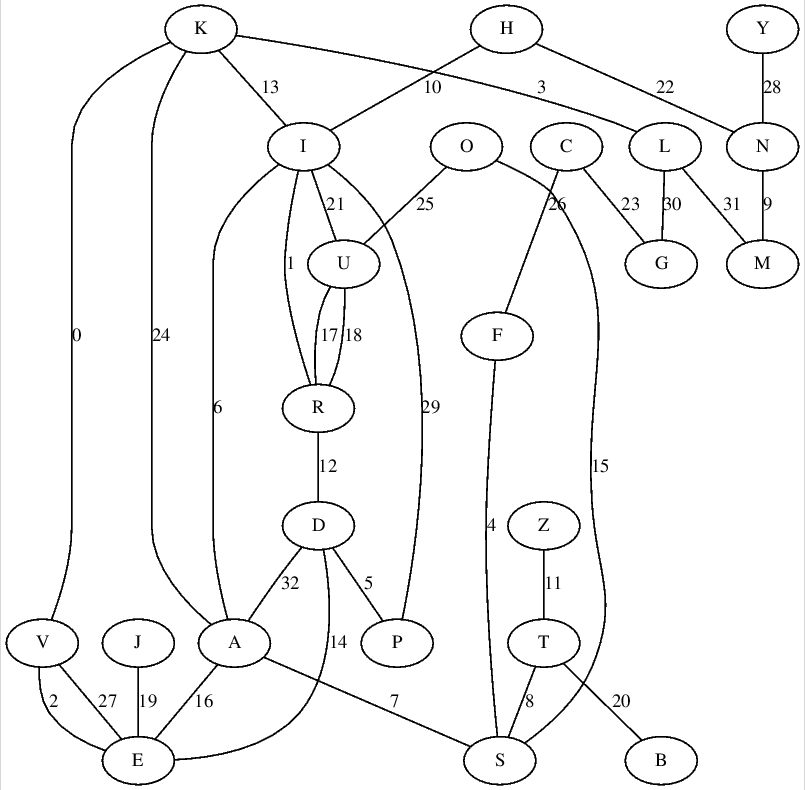
\includegraphics[scale=0.25]{enigma/graph.png}
\end{center}  
Aan de hand van de graph konden we op zoek naar gesloten paden. Door de lengte van de crib waren er heel wat mogelijkheden. We bepaalden voor de letter U 6 gesloten paden. We gingen dan, met elke mogelijke volgorde van rotoren, op zoek naar een $k$ waarvoor een letter invariant bleef op elk van die paden. Hiervoor was een kleine modificatie aan onze ge\"implementeerde Engima machine voldoende. We vonden dat er hiervoor slechts \'e\'en optie was, namelijk rotorvolgorde 420 met als beginstand KSY. De invariante letter was hier de U, wat betekent dat de U door het plugboard niet aangepast wordt. We herhaalden deze test met de letters A, D en I, waarvoor we ook telkens 5 \`a 6 gesloten paden zochten. Hier vonden we ook telkens slechts 1 of 2 resultaten, waaronder altijd \textbf{rotorvolgorde 420} met \textbf{beginstand KSY}. Dit was dus zeker het juiste antwoord. Uit deze resultaten vonden we ook dat het plugboard I en Y verwisselt, en de A en de D niet aanpast. Nu moesten we enkel nog op zoek naar de rest van het plugboard. 

\subsection{Bepalen van het plugboard en ontcijferen van de tekst}
Omdat we een behoorlijk grote crib hadden, waren er voor de meeste letters gesloten paden te vinden in de graph. We konden dus gewoon een versimpelde versie van de voorgaande code draaien voor elke letter met gesloten paden om het plugboard verder te bepalen. Hiervoor hoefden we de test enkel voor de correcte rotorvolgorde en beginstand draaien. De enige letters zonder gesloten paden waren B, J, Q, T, W, X, Y en Z waarbij Q, W en X helemaal niet in de graph voorkwamen, en we al wisten dat Y met I werd omgewisseld. We vonden toch de mappings voor B, Q, W en Z omdat ze elk verwisseld werden met een letter die wel gesloten paden had. We hadden het plugboard dus op J, T en X na bepaald. Er waren nu echter maar 4 mogelijke plugboards over: ofwel werden twee van de drie letters met elkaar gewisseld ofwel werd geen enkele gewisseld. Door de ciphertekst met elk van de vier opties te decipheren, vonden we dat enkel die waarbij J, T en X niet werden aangepast de crib juist ontcijferde en dus juist was. Hiermee hadden we ook het plugboard volledig bepaald en konden we de tekst volledig ontcijferen. Het was een deel uit Die Blechtrommel van G\"unter Grass \footnote{\url{http://www.lawrenceglatz.com/germ3230/texte/grass1.htm}}.




\section{ADFGVX}
\subsection{De opdracht}
De opdracht rond Diffie-Hellman bestond uit twee delen: ten eerste het berekenen van de gezamelijke sleutel en ten tweede het achterhalen van de titels waaruit de geheime sleutels gegenereerd werden.

\subsection{Gezamelijke sleutel: eerste pogingen}
...index calculus, priemontbinding, blabla...

We hebben ook overwogen om met een lijst van titels de sleutels proberen te achterhalen, maar dit was onbegonnen werk aangezien niets geweten was over taal, soort boek, gebruik van hoofdletters en speciale tekens, spaties, ...

\subsection{Gezamelijke sleutel: Pohlig-Hellman}
We stapten vervolgens over op het Pohlig-Hellman algoritme. Dit is in theorie trager dan index calculus, maar veel makkelijker te implementeren. Pohlig-Hellman is namelijk veel makkelijker om volledig automatisch te laten verlopen; het bevat geen vage en lastig te implementeren stappen als "kies een aantal kleine priemgetallen". Ook hoeft slechts van \'e\'en getal de priemontbinding berekend te worden, terwijl dit bij index calculus elke stap gebeurt. We berekenden de priemontbinding van $p-1$ met Wolfram-Alpha. Gezien vele wiskundige pakketten ingebouwde functies hiervoor hebben, vonden we het niet nodig dit met eigen code te berekenen. We hadden hiervoor wel code, alleen werkte deze verschrikkelijk traag.  \\Pohlig-Hellman werkt het snelst met kleine priemfactoren. De grootste priemfactor was $60432007$, wat niet restrictief groot bleek te zijn.  \\ Het algoritme implementeerden we wel helemaal zelf in Python. We baseerden ons op \href{https://www.youtube.com/watch?v=BXFNYVmdtJU}{deze uitleg} van het algoritme. Eerst berekenden we, met inputs de gegeven $A$, $g$ en $p$, voor elke priemfactor $p_i$ (of macht van priemfactor, bij meermaals voorkomende factoren) een $a_i$ zodat $a \equiv a_i (mod\ p_i)$. Hieruit haalden we dan $a\ mod \ (p-1)$ via de Chinese reststelling. Daarna draaiden we het algoritme opnieuw met $B$ om $b$ te bepalen. Gezien voor elke $a_i$ tot $p_i$ mogelijke waardes met trial and error geprobeerd moeten worden, kan het algoritme makkelijk een tiental uur nodig hebben om een resultaat te vinden. We versnelden dit enigszins door het algoritme enkele keren naast elkaar te draaien en verschillende waarden te laten testen. Enkel $a$ of $b$ is voldoende om de gezamelijke sleutel te bepalen, maar we bepaalden ze allebei om ons resultaat te verifi\"eren en omdat we ze toch nodig hebben voor het tweede deel van de opdracht.

\subsection{De titels}
Tsja.

\pagebreak %for style purposes
\begin{appendices}
\section{Oplossingen}
Dit zijn de teksten, waarden en instellingen die we vonden na het decoderen
\subsection{Vigen\`ere}
Volgorde kolomtranspositie: 1, 4, 2, 0, 3, 5 \\
\begingroup
\fontsize{8pt}{10pt}\selectfont
\seqsplit{DEKLEINEERIKLAGJUISTOPHETOGENBLIKDATDITBOEKJEBEGINTINHETOUDEBEDVANGROOTMOEDERPINKSTERBLOMMETDETROONHEMELENDEZIJDENKWASTENENKEEKOVERDERANDVANHETBLANKELAKENDESCHEMERIGEKAMERINHETWASHETUURWAAROPDEKLEINEMENSENNAARBEDGAANHETUURWAARDEGROTEMENSENNIETVANWETENALLEVERTROUWDEDINGENVANDEMUURVERVAGENZOETJESAANINHETGROEIENDEDUISTERENDEWERELDWORDTSTILZOSTILDATZIJZELFSNIETMEERADEMTBUITENSTAPTNOGIEMANDVOORBIJSTAPSTAPZOKLINKTHETENINDEVERTEROEPTEENJONGETJEHOOGENFIJNNAAREENANDERJONGETJEZIJNSTEMKLINKTINDEAVONDENJEDENKTDAARISTOCHEENJONGETJEOPDEWERELDDATNOGNIETINBEDLIGTERIKLAGSTILTEKIJKENNAARHETRAAMINDEVERTEENNAARDESCHEMERENDEPORTRETTENVANDEMUURHETISNETDACHTHIJOFERIETSGEBEURENGAATENMISSCHIENGAATEROOKWELIETSGEBEURENENHIJBESLOOTOMNUEENSNIETGELIJKOPANDEREAVONDENINSLAAPTEVALLENMAARGOEDOPTELETTENOFERMISSCHIENIETSGEBEURENGINGNUWASDAAREENGOEDMIDDELVOORWANTONDERZIJNHOOFDKUSSENLAGEENBOEKJESOLMSBEKNOPTENATUURLIJKEHISTORIEGEHETENENERIKMOESTDAARVOORMORGENALLEINSECTENUITKENNENHIJHADERDEZEHELEWOENSDAGMIDDAGUITZITTENLERENENWASTOTAANDEMEIKEVERSGEKOMENMORGENOCHTENDONDERHETSPEELKWARTIERZOUHIJDEMEIKEVERSERBIJNEMENLAATEENSKIJKENMOMPELDEERIKHOEVEELPOTENHEEFTEENWESPOOKALWEERZESDEOGENZIJNAPARTVERSTELBAARENSTAANVOORINDEKOPMOOIZIJLEVENNIETINKORVENGELIJKDEBIJENMAARJAWAARLEVENZIJDANZIJZULLENAPARTLEVENDENKIKNUDATDOETEROOKNIETTOEZIJBEHORENTOTDEFAMILIEDERVLIESVLEUGELIGENENHEBBENGEKNIKTESPRIETENENHOESTAATHETMETDEVLINDERS}
\endgroup
\subsection{Playfair}
\begingroup
\fontsize{8pt}{10pt}\selectfont
\seqsplit{AWELXLKNOWNSCIENTISTSOMESAYITWASBERTRANDRUSXSELXLONCEGAVEAPUBLICLECTUREONASTRONOMYHEDESCRIBEDHOWTHEXEARTHORBITSAROUNDTHESUNANDHOWTHESUNINTURNORBITSAROUNDTHECENTEROFAVASTCOLXLECTIONOFSTARSCALXLEDOURGALAXYATXTHEXENDOFTHELECTUREALITXTLEOLDLADYATXTHEBACKOFTHEROXOMGOTUPANDSAIDWHATYOUHAVETOLDUSISRUBXBISHTHEWORLDISREALXLYAFLATPLATESUPXPORTEDONTHEBACKOFAGIANTXTORTOISETHESCIENTISTGAVEASUPERIORSMILEBEFOREREPLYINGWHATISTHETORTOISESTANDINGONYOUREVERYCLEVERYOUNGMANVERYCLEVERSAIDTHEOLDLADYBUTITSTURTLESALXLTHEWAYDOWNMOSTPEOPLEWOULDFINDTHEPICTUREOFOURUNIVERSEASANINFINITETOWEROFTORTOISESRATHERXRIDICULOUSBUTWHYDOWETHINKWEKNOWBETXTERWHATDOWEKNOWABOUTXTHEUNIVERSEANDHOWDOWEKNOWITWHEREDIDTHEUNIVERSECOMEFROMANDWHEREISITGOINGDIDTHEUNIVERSEHAVEABEGINXNINGANDIFSOWHATHAPXPENEDBEFORETHENWHATISTHENATUREOFTIMEWILXLITEVERCOMETOANENDCANWEGOBACKINTIMERECENTBREAKTHROUGHSINPHYSICSMADEPOSXSIBLEINPARTBYFANTASTICNEWTECHNOLOGIESXSUGXGESTANSWERSTOSOMEOFTHESELONGSTANDINGQUESTIONSXSOMEDAYTHESEANSWERSMAYSEXEMASOBVIOUSTOUSASTHEXEARTHORBITINGTHESUNORPERHAPSASRIDICULOUSASATOWEROFTORTOISESONLYTIMEWHATEVERTHATMAYBEWILXLTELXLASLONGAGOASTHREXEHUNDREDANDFOURTYBCTHEGREXEKPHILOSOPHERARISTOTLEINHISBOXOKONTHEHEAVENSWASABLETOPUTFORWARDTWOGOXODARGUMENTSFORBELIEVINGTHATXTHEXEARTHWASAROUNDSPHERERATHERTHANAHATPLATEFIRSTHEREALIZEDTHATECLIPSESOFTHEMOXONWERECAUSEDBYTHEXEARTHCOMINGBETWEXENTHESUNANDTHEMOXONTHEXEARTHSXSHADOWONTHEMOXONWASALWAYSROUNDWHICHWOULDBETRUEONLYIFTHEXEARTHWASXSPHERICALIFTHEXEARTHXHADBEXENAFLATDISKTHESHADOWXWOULDHAVEBEXENELONGATEDANDELXLIPTICALUNLESXSTHEXECLIPSEALWAYSOCXCURXREDATATIMEWHENTHESUNWASDIRECTLYUNDERTHECENTEROFTHEDISKSECONDTHEGREXEKSKNEWFROMTHEIRTRAVELSTHATXTHENORTHSTARAPXPEAREDLOWERINTHESKYWHENVIEWEDINTHESOUTHTHANITDIDINMORENORTHERLYREGIONSXSINCETHENORTHSTARLIESOVERTHENORTHPOLEITAPXPEARSTOBEDIRECTLYABOVEANOBSERVERATXTHENORTHPOLEBUTXTOSOMEONELOXOKINGFROMTHEXEQUATORITAPXPEARSTOLIEIUSTATXTHEHORIZONFROMTHEDIFXFERENCEINTHEAPXPARENTPOSITIONOFTHENORTHSTARINEGYPTANDGREXECEARISTOTLEXEVENQUOTEDANESTIMATETHATXTHEDISTANCEAROUNDTHEXEARTHWASFOURHUNDREDTHOUSANDSTADIAITISNOTKNOWNEXACTLYWHATLENGTHASTADIUMWASBUTITMAYHAVEBEXENABOUTXTWOHUNDREDYARDSWHICHWOULDMAKEARISTOTLESESTIMATEABOUTXTWICETHECURXRENTLYACXCEPTEDFIGURETHEGREXEKSEVENHADATHIRDARGUMENTXTHATXTHEXEARTHMUSTBEROUNDFORWHYELSEDOESONEFIRSTSEXETHESAILSOFASHIPCOMINGOVERTHEHORIZONANDONLYLATERSEXETHEHULXLARISTOTLETHOUGHTXTHEXEARTHWASXSTATIONARYANDTHATXTHESUNTHEMOXONTHEPLANETSANDTHESTARSMOVEDINCIRCULARORBITSABOUTXTHEXEARTHXHEBELIEVEDTHISBECAUSEHEFELTFORMYSTICALREASONSTHATXTHEXEARTHWASTHECENTEROFTHEUNIVERSEANDTHATCIRCULARMOTIONWASTHEMOSTPERFECTXTHISIDEAWASELABORATEDBYPTOLEMYINTHESECONDCENTURYADINTOACOMPLETECOSMOLOGICALMODELTHEXEARTHSTOXODATXTHECENTERSURXROUNDEDBYEIGHTSPHERESTHATCARXRIEDTHEMOXONTHESUNTHESTARSANDTHEFIVEPLANETSKNOWNATXTHETIMEMERCURYVENUSMARSIUPITERANDSATURNX}
\endgroup
\subsection{ADFGVX}
Volgorde kolomtranspositie: 1, 3, 2, 0 of 3, 1, 0, 2 \\
\begingroup
\fontsize{8pt}{10pt}\selectfont
\seqsplit{LANNEE1866FUTMARQUEEPARUNEVENEMENTBIZARREUNPHENOMENEINEXPLIQUEETINEXPLICABLEQUEPERSONNENASANSDOUTEOUBLIESANSPARLERDESRUMEURSQUIAGITAIENTLESPOPULATIONSDESPORTSETSUREXCITAIENTLESPRITPUBLICALINTERIEURDESCONTINENTSLESGENSDEMERFURENTPARTICULIEREMENTEMUSLESNEGOCIANTSARMATEURSCAPITAINESDENAVIRESSKIPPERSETMASTERSDELEUROPEETDELAMERIQUEOFFICIERSDESMARINESMILITAIRESDETOUSPAYSETAPRESEUXLESGOUVERNEMENTSDESDIVERSETATSDESDEUXCONTINENTSSEPREOCCUPERENTDECEFAITAUPLUSHAUTPOINTENEFFETDEPUISQUELQUETEMPSPLUSIEURSNAVIRESSETAIENTRENCONTRESSURMERAVECUNECHOSEENORMEUNOBJETLONGFUSIFORMEPARFOISPHOSPHORESCENTINFINIMENTPLUSVASTEETPLUSRAPIDEQUUNEBALEINELESFAITSRELATIFSACETTEAPPARITIONCONSIGNESAUXDIVERSLIVRESDEBORDSACCORDAIENTASSEZEXACTEMENTSURLASTRUCTUREDELOBJETOUDELETREENQUESTIONLAVITESSEINOUEDESESMOUVEMENTSLAPUISSANCESURPRENANTEDESALOCOMOTIONLAVIEPARTICULIEREDONTILSEMBLAITDOUESICETAITUNCETACEILSURPASSAITENVOLUMETOUSCEUXQUELASCIENCEAVAITCLASSESJUSQUALORSNICUVIERNILACEPEDENIMDUMERILNIMDEQUATREFAGESNEUSSENTADMISLEXISTENCEDUNTELMONSTREAMOINSDELAVOIRVUCEQUISAPPELLEVUDELEURSPROPRESYEUXDESAVANTSAPRENDRELAMOYENNEDESOBSERVATIONSFAITESADIVERSESREPRISESENREJETANTLESEVALUATIONSTIMIDESQUIASSIGNAIENTACETOBJETUNELONGUEURDEDEUXCENTSPIEDSETENREPOUSSANTLESOPINIONSEXAGEREESQUILEDISAIENTLARGEDUNMILLEETLONGDETROISONPOUVAITAFFIRMERCEPENDANTQUECETETREPHENOMENALDEPASSAITDEBEAUCOUPTOUTESLESDIMENSIONSADMISESJUSQUACEJOURPARLESICHTYOLOGISTESSILEXISTAITTOUTEFOISORILEXISTAITLEFAITENLUIMEMENETAITPLUSNIABLEETAVECCEPENCHANTQUIPOUSSEAUMERVEILLEUXLACERVELLEHUMAINEONCOMPRENDRALEMOTIONPRODUITEDANSLEMONDEENTIERPARCETTESURNATURELLEAPPARITIONQUANTALAREJETERAURANGDESFABLESILFALLAITYRENONCERENEFFETLE20JUILLET1866LESTEAMERGOVERNORHIGGINSONDECALCUTTAANDBURNACHSTEAMNAVIGATIONCOMPANYAVAITRENCONTRECETTEMASSEMOUVANTEACINQMILLESDANSLESTDESCTESDELAUSTRALIELECAPITAINEBAKERSECRUTTOUTDABORDENPRESENCEDUNECUEILINCONNUILSEDISPOSAITMEMEAENDETERMINERLASITUATIONEXACTEQUANDDEUXCOLONNESDEAUPROJETEESPARLINEXPLICABLEOBJETSELANCERENTENSIFFLANTACENTCINQUANTEPIEDSDANSLAIRDONCAMOINSQUECETECUEILNEFTSOUMISAUXEXPANSIONSINTERMITTENTESDUNGEYSERLEGOVERNORHIGGINSONAVAITAFFAIREBELETBIENAQUELQUEMAMMIFEREAQUATIQUEINCONNUJUSQUELAQUIREJETAITPARSESEVENTSDESCOLONNESDEAUMELANGEESDAIRETDEVAPEURPAREILFAITFUTEGALEMENTOBSERVELE23JUILLETDELAMEMEANNEEDANSLESMERSDUPACIFIQUEPARLECRISTOBALCOLONDEESTINDIAANDPACIFICSTEAMNAVIGATIONCOMPANYDONCCECETACEEXTRAORDINAIREPOUVAITSETRANSPORTERDUNENDROITAUNAUTREAVECUNEVELOCITESURPRENANTEPUISQUEATROISJOURSDINTERVALLELEGOVERNORHIGGINSONETLECRISTOBALCOLONLAVAIENTOBSERVEENDEUXPOINTSDELACARTESEPARESPARUNEDISTANCEDEPLUSDESEPTCENTSLIEUESMARINESQUINZEJOURSPLUSTARDADEUXMILLELIEUESDELALHELVETIADELACOMPAGNIENATIONALEETLESHANNONDUROYALMAILMARCHANTACONTREBORDDANSCETTEPORTIONDELATLANTIQUECOMPRISEENTRELESETATSUNISETLEUROPESESIGNALERENTRESPECTIVEMENTLEMONSTREPAR4215DELATITUDENORDET6035DELONGITUDEALOUESTDUMERIDIENDEGREENICHDANSCETTEOBSERVATIONSIMULTANEEONCRUTPOUVOIREVALUERLALONGUEURMINIMUMDUMAMMIFEREAPLUSDETROISCENTCINQUANTEPIEDSANGLAISPUISQUELESHANNONETLHELVETIAETAIENTDEDIMENSIONINFERIEUREALUIBIENQUILSMESURASSENTCENTMETRESDELETRAVEALETAMBOTORLESPLUSVASTESBALEINESCELLESQUIFREQUENTENTLESPARAGESDESLESALEOUTIENNESLEKULAMMAKETLUMGULLICKNONTJAMAISDEPASSELALONGUEURDECINQUANTESIXMETRESSIMEMEELLESLATTEIGNENTCESRAPPORTSARRIVESCOUPSURCOUPDENOUVELLESOBSERVATIONSFAITESABORDDUTRANSATLANTIQUELEPEREIREUNABORDAGEENTRELETNADELALIGNEINMANETLEMONSTREUNPROCESVERBALDRESSEPARLESOFFICIERSDELAFREGATEFRANAISELANORMANDIEUNTRESSERIEUXRELEVEMENTOBTENUPARLETATMAJORDUCOMMODOREFITZJAMESABORDDULORDCLYDEEMURENTPROFONDEMENTLOPINIONPUBLIQUEDANSLESPAYSDHUMEURLEGEREONPLAISANTALEPHENOMENEMAISLESPAYSGRAVESETPRATIQUESLANGLETERRELAMERIQUELALLEMAGNESENPREOCCUPERENTVIVEMENT}
\endgroup
\subsection{Enigma}
Rotorvolgorde: 420 \\
Beginstand: KSY \\
Plugboard:  AKEDCHGFYJBLWNZPSRQTUVMXIO \\
Verwisselingen in plugboard: B-K, C-E, F-H, I-Y, M-W, O-Z, Q-S \\
\begingroup
\fontsize{8pt}{10pt}\selectfont
\seqsplit{VIELSPASSMITDIESERUEBUNGAUFENIGMAZUGEGEBENICHBININSASSEEINERHEILUNDPFLEGEANSTALTMEINPFLEGERBEOBACHTETMICHLASSTMICHKAUMAUSDEMAUGEDENNINDERTURISTEINGUCKLOCHUNDMEINESPFLEGERSAUGEISTVONJENEMBRAUNWELCHESMICHDENBLAUAUGIGENNICHTDURCHSCHAUENKANNMEINPFLEGERKANNALSOGARNICHTMEINFEINDSEINLIEBGEWONNENHABEICHIHNERZAHLEDEMGUCKERHINTERDERTURSOBALDERMEINZIMMERBETRITTBEGEBENHEITENAUSMEINEMLEBENDAMITERMICHTROTZDESIHNHINDERNDENGUCKLOCHESKENNENLERNTDERGUTESCHEINTMEINEERZAHLUNGENZUSCHATZENDENNSOBALDICHIHMETWASVORGELOGENHABEZEIGTERMIRUMSICHERKENNTLICHZUGEBENSEINNEUESTESKNOTENGEBILDEOBEREINKUNSTLERISTBLEIBEDAHINGESTELLTEINEAUSSTELLUNGSEINERKREATIONENWURDEJEDOCHVONDERPRESSEGUTAUFGENOMMENWERDENAUCHEINIGEKAUFERHERBEILOCKENERKNOTETORDINAREBINDFADENDIEERNACHDENBESUCHSSTUNDENINDENZIMMERNSEINERPATIENTENSAMMELTUNDENTWIRRTZUVIELSCHICHTIGVERKNORPELTENGESPENSTERNTAUCHTDIESEDANNINGIPSLASSTSIEERSTARRENUNDSPIESSTSIEMITSTRICKNADELNDIEAUFHOLZSOCKELCHENBEFESTIGTSINDOFTSPIELTERMITDEMGEDANKENSEINEWERKEFARBIGZUGESTALTENICHRATEDAVONABWEISEAUFMEINWEISSLACKIERTESMETALLBETTHINUNDBITTEIHNSICHDIESESVOLLKOMMENSTEBETTBUNTBEMALTVORZUSTELLENENTSETZTSCHLAGTERDANNSEINEPFLEGERHANDEUBERDEMKOPFZUSAMMENVERSUCHTINETWASZUSTARREMGESICHTALLENSCHRECKENGLEICHZEITIGAUSDRUCKZUGEBENUNDNIMMTABSTANDVONSEINENFARBIGENPLANENMEINWEISSLACKIERTESMETALLENESANSTALTSBETTISTALSOEINMASSSTABMIRISTESSOGARMEHRMEINBETTISTDASENDLICHERREICHTEZIELMEINTROSTISTESUNDKONNTEMEINGLAUBEWERDENWENNMIRDIEANSTALTSLEITUNGERLAUBTEEINIGEANDERUNGENVORZUNEHMENDASBETTGITTERMOCHTEICHERHOHENLASSENDAMITMIRNIEMANDMEHRZUNAHETRITTEINMALINDERWOCHEUNTERBRICHTEINBESUCHSTAGMEINEZWISCHENWEISSENMETALLSTABENGEFLOCHTENESTILLEDANNKOMMENSIEDIEMICHRETTENWOLLENDENENESSPASSMACHTMICHZULIEBENDIESICHINMIRSCHATZENACHTENUNDKENNENLERNENMOCHTENWIEBLINDNERVOSWIEUNERZOGENSIESINDKRATZENMITIHRENFINGERNAGELSCHERENANMEINEMWEISSLACKIERTENBETTGITTERKRITZELNMITIHRENKUGELSCHREIBERNUNDBLAUSTIFTENDEMLADELANGGEZOGENEUNANSTANDIGESTRICHMANNCHENMEINANWALTSTULPTJEDESMALSOBALDERMITSEINEMHALLODASZIMMERSPRENGTDENNYLONHUTUBERDENLINKENPFOSTENAMFUSSENDEMEINESBETTESSOLANGESEINBESUCHWAHRTUNDANWALTEWISSENVIELZUERZAHLENRAUBTERMIRDURCHDIESENGEWALTAKTDASGLEICHGEWICHTUNDDIEHEITERKEITNACHDEMMEINEBESUCHERIHREGESCHENKEAUFDEMWEISSENMITWACHSTUCHBEZOGENENTISCHCHENUNTERDEMANEMONENAQUARELLDEPONIERTHABENNACHDEMESIHNENGELUNGENISTMIRIHREGERADELAUFENDENODERGEPLANTENRETTUNGSVERSUCHEZUUNTERBREITENUNDMICHDENSIEUNERMUDLICHRETTENWOLLENVOMHOHENSTANDARDIHRERNACHSTENLIEBEZUUBERZEUGENFINDENSIEWIEDERSPASSANDEREIGENENEXISTENZUNDVERLASSENMICHDANNKOMMTMEINPFLEGERUMZULUFTENUNDDIEBINDFADENDERGESCHENKPACKUNGENEINZUSAMMELNOFTMALSFINDETERNACHDEMLUFTENNOCHZEITANMEINEMBETTSITZENDBINDFADENAUFDROSELNDSOLANGESTILLEZUVERBREITENBISICHDIESTILLEBRUNOUNDBRUNODIESTILLENENNEBRUNOMUNSTERBERGICHMEINEJETZTMEINENPFLEGERLASSEDASWORTSPIELHINTERMIRKAUFTEAUFMEINERECHNUNGFUNFHUNDERTBLATTSCHREIBPAPIERBRUNODERUNVERHEIRATETKINDERLOSISTUNDAUSDEMSAUERLANDSTAMMTWIRDSOLLTEDERVORRATNICHTREICHENDIEKLEINESCHREIBWARENHANDLUNGINDERAUCHKINDERSPIELZEUGVERKAUFTWIRDNOCHEINMALAUFSUCHENUNDMIRDENNOTWENDIGENUNLINIERTENPLATZFURMEINHOFFENTLICHGENAUESERINNERUNGSVERMOGENBESCHAFFENNIEMALSHATTEICHMEINEBESUCHERETWADENANWALTODERKLEPPUMDIESENDIENSTBITTENKONNENBESORGTEMIRVERORDNETELIEBEHATTEDENFREUNDENSICHERVERBOTENETWASSOGEFAHRLICHESWIEUNBESCHRIEBENESPAPIERMITZUBRINGENUNDMEINEMUNABLASSIGSILBENAUSSCHEIDENDENGEISTZUMGEBRAUCHFREIZUGEBENALSICHZUBRUNOSAGTEACHBRUNOWURDESTDUMIRFUNFHUNDERTBLATTUNSCHULDIGESPAPIERKAUFENANTWORTETEBRUNOZURZIMMERDECKEBLICKENDUNDSEINENZEIGEFINGEREINENVERGLEICHHERAUSFORDERNDINDIEGLEICHERICHTUNGSCHICKENDSIEMEINENWEISSESPAPIERHERROSKAR}
\endgroup
\subsection{Diffie-Hellman}
Gezamenlijke sleutel: \\76755567381519549143666616401510211097526907381540 \\ \\
Geheime sleutels: \\
29118405404220459917506399212097843017814710983140 (Annie)\\
42146349908839709291089275597341571419432358218840 (Boris)

\section{De code uitvoeren}
De code die we gebruikten om onze oplossingen te vinden, is geschreven in Python en in Go. In ons ingestuurde project is alle geschreven code te vinden, ook die die uiteindelijk niet gebruikt werd om het resultaat te vinden. Een subsectie van de code, met enkele vereenvoudigingen, is te vinden in de map solutionCode. Hier is de code verdeeld in een map met alle Pythonscripts en een map met alle Go-code. Om de Pythoncode te runnen volstaat het "python3 *filenaam*" uit te voeren. Merk op dat Python3 vereist is, sommige code werkt niet onder Python2. Om de Go-code uit te voeren is wat meer setup vereist. Op Ubuntu kan Go ge\"installeerd worden via "sudo apt-get install golang". Voer daarna "export GOPATH=*pathtorootfolder*/CodingTheory/solutionCode/Go" uit, waarbij *pathtorootfolder* vervangen wordt met het pad naar waar de map CodingTheory uitgepakt is. Vervolgens volstaat het om in CodingTheory/solutionCode/Go/src/CodingTheory "go build" uit te voeren om een executable aan te maken. Wat volgt is een oplijsting van uit te voeren code per opdracht en wat het reconstrueert.

\begin{enumerate}
  \item Vigen\`ere: Python/vigenere/vigerene.py: Maakt eerst de kolomtranspositie ongedaan (toont alle 6 de mogelijkheden gevonden door onze code) en maakt daarna de monoalfabetische substitutie ongedaan.
  \item Playfair: Python/playfair/playfair.py: Vindt met een vaste seed vrij snel de juiste brontekst met het Churn algoritme.
  \item ADFGVX: Python/ADFGVX/ADFGVX.py: Maakt de kolomtranspositie ongedaan (toont 4 mogelijkheden waaronder de 2 correcte). De rest werd met de hand opgelost.
  \item Enigma: Go/src/CodingTheory/CodingTheory (aan te maken met "go build"): Vindt rotorvolgorde en beginsettings, decodeert daarna de volledige tekst (met vooraf ingesteld plugboard). Om het bepalen van het plugboard te reconstrueren dienen lijnen code in main.go (uit)gecomment te worden, zoals in de code zelf is aangegeven.
  \item Diffie-Hellman: Python/diffiehellman/diffiehellman.py: Dit begint met het uitvoeren van het Pohlig-Hellman algoritme, maar dit is standaard uitgecomment gezien dit meer dan een halve dag runtime vergt. Standaard worden enkel de private keys uitgerekend met de Chinese reststelling, en wordt de correctheid van deze keys en de gezamenlijke key nagegaan. textSolver.py probeert de boektitel te vinden. Deze code eindigt niet en vindt voor zover wij weten geen correct resultaat.
\end{enumerate}
\end{appendices}

\end{document}
